表\ref{tab:initial}给出同一500条测试新闻上的标题生成结果。预训练后微调的ROUGE-L为28.77，随机初始化微调为9.43，前者高出19.34个分值点。与同输入抽取基线相比，预训练后微调高出5.85个分值点。

\begin{table}[H]
\centering\small
\caption{标题生成对照结果}\label{tab:initial}
\begin{tabularx}{\linewidth}{Y r r r}
\toprule 方法 & ROUGE-1 & ROUGE-2 & ROUGE-L \\ \midrule
首句前32字符 & 26.28 & 14.98 & 22.92 \\
仅预训练 & 2.89 & 1.25 & 2.77 \\
随机初始化微调 & 9.56 & 3.71 & 9.43 \\
预训练后微调 & 30.81 & 17.99 & 28.77 \\
\bottomrule
\end{tabularx}
\end{table}

图\ref{fig:sft}比较两组微调损失，两个子图分别设置纵轴范围。

\begin{figure}[H]

\centering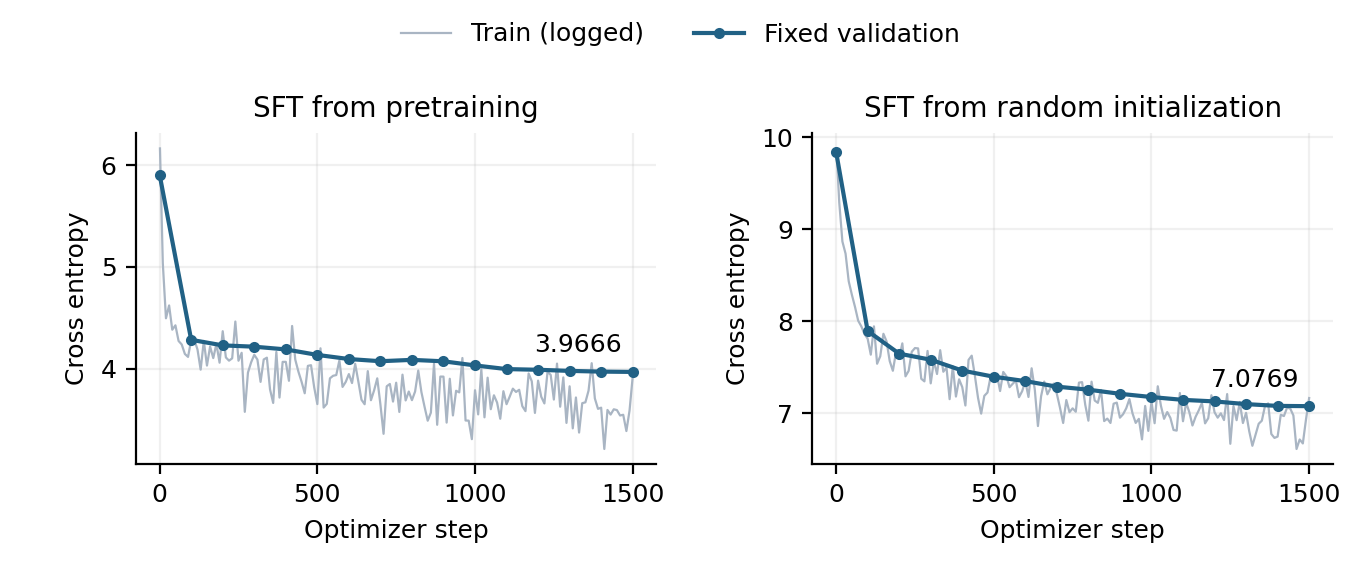
\includegraphics[width=\linewidth]{generated/sft_comparison.png}

\caption{标题微调损失曲线}\label{fig:sft}

\end{figure}

两组最佳验证交叉熵分别为3.9666和7.0769，均出现在第1500步。仅预训练模型的标题得分较低，监督微调有助于学习标题格式和信息选择。预训练组还使用了额外预训练计算，随机初始化组沿用同一微调配置，上述差异反映当前设置下初始化与训练方案的共同影响。

在相同的标题监督范围下，两组固定验证困惑度分别为52.81和1184.25。预训练组更容易利用已有语言表示拟合标题目标。只有预训练时，模型尚未充分适配“读正文、生成标题”的任务格式，因此损失与生成评测共同支持预训练和任务监督分别发挥作用的解释。
